\documentclass[10pt,a4paper]{article}
\usepackage[T1]{fontenc}
\usepackage{lmodern}
\usepackage[margin=2cm]{geometry}
\usepackage{booktabs}
\usepackage{amsmath}
\usepackage{amssymb}
\usepackage{tikz}
\usetikzlibrary{arrows.meta, positioning, fit, backgrounds, calc, decorations.pathreplacing}
\usepackage{float}
\usepackage[hidelinks]{hyperref}
\usepackage{listings}
\usepackage{xcolor}
\newcommand{\NCells}{43}
\newcommand{\NNorm}{42}
\newcommand{\Seeds}{3}
\newcommand{\NTraces}{15}
\newcommand{\NormTIDE}{0.379}
\newcommand{\NormARC}{0.306}
\newcommand{\NormSthree}{0.334}
\newcommand{\NormLFU}{$-0.257$}
\newcommand{\WinsTIDE}{24}
\newcommand{\GeARC}{34}
\newcommand{\Worst}{$-0.54$}
\newcommand{\WorstCell}{phases, $c=20181$}
\newcommand{\GapShare}{37}
\newcommand{\AdvGain}{+48.6}
\newcommand{\GainLifecycle}{+0.9}
\newcommand{\GainCycle}{+34.5}
\newcommand{\GainPhases}{+10.6}
\newcommand{\PFifty}{15}
\newcommand{\PNineNineMax}{30}
\newcommand{\RpsMin}{45}
\newcommand{\RpsMax}{123}
\newcommand{\TrainPct}{21}


\definecolor{cARC}{HTML}{1E88E5}
\definecolor{cTIDE}{HTML}{D81B60}
\definecolor{cGray}{HTML}{9E9E9E}
\definecolor{cGreen}{HTML}{43A047}
\definecolor{cOrange}{HTML}{FB8C00}
\lstset{basicstyle=\ttfamily\small, columns=fullflexible, keepspaces=true}

\newcommand{\code}[1]{\texttt{#1}}

\title{How TIDE works\\\Large A plain-English and technical walkthrough}
\author{Cache replacement project}
\date{\today}

\begin{document}
\maketitle
\tableofcontents

\section{The problem in one paragraph}
A cache is a small, fast storage area that holds a limited number of items so that repeat requests for
them are served quickly instead of going to slow storage. When the cache is full and a new item arrives,
something already in the cache has to be thrown out to make room. Which item to throw out is the
\emph{eviction} decision, and it is the only thing that separates a good cache policy from a bad one:
every policy stores the same items, they just disagree about which one to evict. TIDE is a new eviction
policy. It wraps a well-known policy called ARC and adds a small, constantly learning model that makes
the eviction choice ARC would otherwise make on its own. This document explains, in order: what ARC
does, why it is not enough on its own, what TIDE adds, exactly what numbers it computes for each
candidate, the exact network and how it trains itself while the cache is running, and how it protects
itself from its own mistakes. Every rule stated here is the rule implemented in \code{tide.py} and
\code{policies.py}; there is no simplification that changes behaviour.

\section{Baseline: what ARC does on its own}
ARC (\emph{Adaptive Replacement Cache}, Megiddo \& Modha, 2003) keeps four lists instead of the one list a
simple cache uses:

\begin{itemize}
  \item \textbf{T1}: items currently in the cache that have been requested \emph{once recently}.
  \item \textbf{T2}: items currently in the cache that have been requested \emph{at least twice}, i.e.\ they
        have shown up again since they were last considered "new".
  \item \textbf{B1}: a \emph{ghost list} — not actual data, just a memory of keys recently evicted from T1.
  \item \textbf{B2}: a ghost list of keys recently evicted from T2.
\end{itemize}

The point of B1 and B2 is that ARC can notice when it evicted something too early. If a key that was in
B1 comes back, that is evidence ARC is throwing away "recency" items too fast, so it grows T1 at T2's
expense. If a key from B2 comes back, ARC was throwing away "frequency" items too fast, so it shrinks T1.
This growing and shrinking is controlled by a single number, $p$, which is the target size of T1.

\begin{figure}[H]
\centering
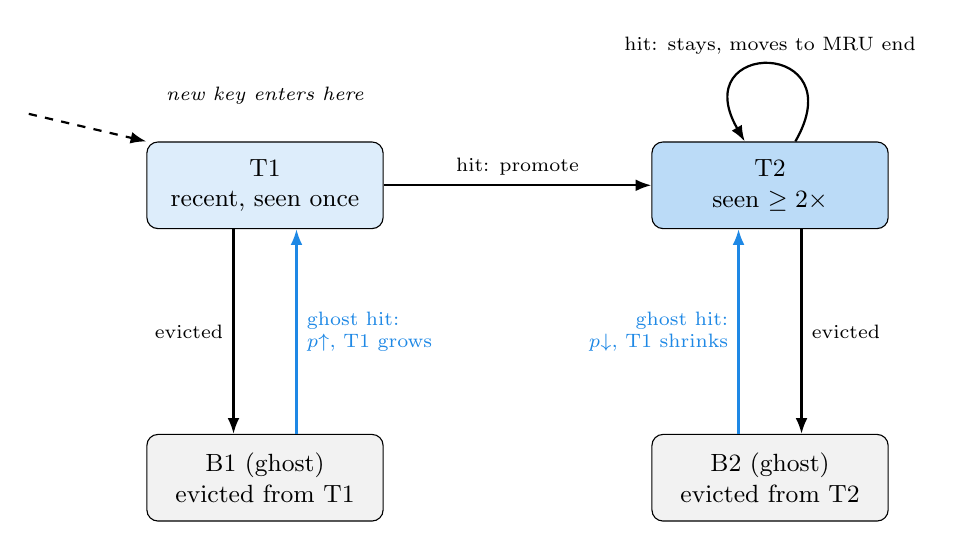
\begin{tikzpicture}[
  box/.style={draw, rounded corners, minimum width=3.0cm, minimum height=1.1cm, align=center, font=\small},
  lbl/.style={font=\scriptsize, align=center},
  arr/.style={-{Latex[length=2mm]}, thick}
]
\node[box, fill=cARC!15] (t1) {T1\\recent, seen once};
\node[box, fill=cARC!30, right=3.4cm of t1] (t2) {T2\\seen $\ge 2\times$};
\node[box, fill=gray!10, below=2.6cm of t1] (b1) {B1 (ghost)\\evicted from T1};
\node[box, fill=gray!10, below=2.6cm of t2] (b2) {B2 (ghost)\\evicted from T2};

\draw[arr] (t1) -- node[lbl, above]{hit: promote} (t2);
\draw[arr] (t2) to[out=60,in=120,looseness=6] node[lbl, above]{hit: stays, moves to MRU end} (t2);
\draw[arr] ($(t1.south)+(-0.4,0)$) -- node[lbl, left]{evicted} ($(b1.north)+(-0.4,0)$);
\draw[arr] ($(t2.south)+(0.4,0)$) -- node[lbl, right]{evicted} ($(b2.north)+(0.4,0)$);
\draw[arr, cARC, thick] ($(b1.north)+(0.4,0)$) -- node[lbl, right, cARC, align=left]{ghost hit:\\$p{\uparrow}$, T1 grows} ($(t1.south)+(0.4,0)$);
\draw[arr, cARC, thick] ($(b2.north)+(-0.4,0)$) -- node[lbl, left, cARC, align=right]{ghost hit:\\$p{\downarrow}$, T1 shrinks} ($(t2.south)+(-0.4,0)$);
\node[lbl, above=0.35cm of t1, font=\scriptsize\itshape] {new key enters here};
\draw[arr, dashed] ($(t1.north)+(-3.0,0.35)$) -- (t1.north west);
\end{tikzpicture}
\caption{ARC's four lists. T1 and T2 hold the actual cached items; B1 and B2 remember only the \emph{keys}
of recently evicted items, so ARC can tell whether an eviction was a mistake.}
\end{figure}

Formally, on a ghost hit:
\[
\text{B1 hit:}\quad p \leftarrow \min\!\Big(c,\; p + \max\!\big(1, \tfrac{|B2|}{|B1|}\big)\Big)
\qquad
\text{B2 hit:}\quad p \leftarrow \max\!\Big(0,\; p - \max\!\big(1, \tfrac{|B1|}{|B2|}\big)\Big)
\]
where $c$ is the cache capacity. When something must be evicted, ARC's \code{REPLACE} rule decides
\emph{which list} loses an item: it evicts from T1 if T1 is bigger than its target $p$ (or a tie-break
case), otherwise from T2. Whichever list is chosen, plain ARC always evicts that list's
\emph{least-recently-used} (LRU) item — the one nobody has asked for in the longest time.

\paragraph{Where ARC falls short.} ARC decides \emph{which list} to shrink well, using real feedback, but
inside that list it falls back to plain "oldest first", which cannot see repeating patterns. Two examples
that break it, both measured on real traces during this project:
\begin{itemize}
  \item \textbf{A loop bigger than the cache.} If items $1, 2, \dots, 17$ are requested over and over
        with a cache of size 16, ARC (and LRU) get a \textbf{0\% hit rate} — the item ARC always evicts
        is always the very next one requested. TIDE gets that same trace above 40\% higher than ARC and
        LRU (see \code{test\_tide.py::test\_learns\_loop}).
  \item \textbf{A one-time scan.} A burst of never-repeated keys pushes every genuinely useful item out
        of T1's LRU end before ARC even realises the burst is over.
\end{itemize}

\section{What TIDE adds: a learned victim}
TIDE keeps ARC's four lists and its $p$ update rule completely unchanged. The only thing that changes is
\emph{which item} is evicted from the list ARC picked. Instead of always taking the oldest item, TIDE
scores a handful of candidates with a small neural network and evicts whichever one the network thinks
is safest to lose --- i.e.\ the one that will not be needed again for the longest time.

\begin{figure}[H]
\centering
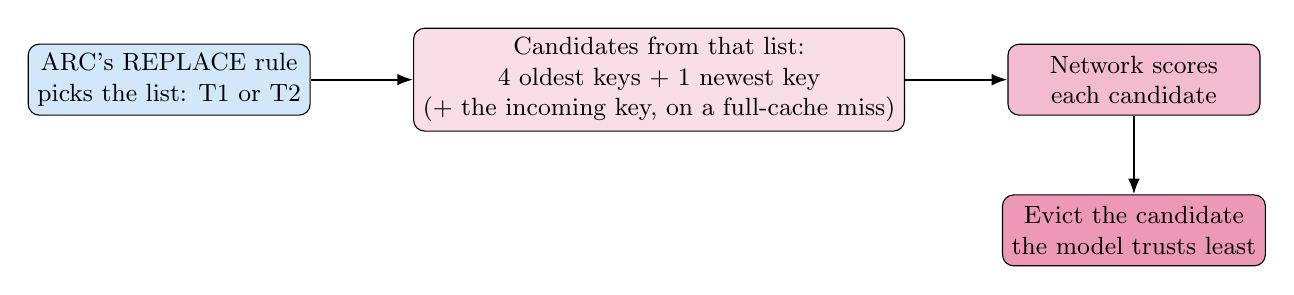
\begin{tikzpicture}[
  box/.style={draw, rounded corners, minimum height=0.9cm, align=center, font=\small},
  arr/.style={-{Latex[length=2mm]}, thick}
]
\node[box, fill=cARC!20, minimum width=3.4cm] (arc) {ARC's REPLACE rule\\picks the list: T1 or T2};
\node[box, fill=cTIDE!15, right=1.3cm of arc, minimum width=5.2cm] (cand)
  {Candidates from that list:\\4 oldest keys + 1 newest key\\(+ the incoming key, on a full-cache miss)};
\node[box, fill=cTIDE!30, right=1.3cm of cand, minimum width=3.2cm] (net) {Network scores\\each candidate};
\node[box, fill=cTIDE!45, below=1.0cm of net, minimum width=3.2cm] (pick) {Evict the candidate\\the model trusts least};
\draw[arr] (arc) -- (cand);
\draw[arr] (cand) -- (net);
\draw[arr] (net) -- (pick);
\end{tikzpicture}
\caption{TIDE's decision pipeline for one eviction. ARC still decides the list; TIDE only decides the
victim within it.}
\end{figure}

\subsection{Exactly which candidates are scored}
For the list $L$ that ARC's rule selected, TIDE builds a candidate set of up to six keys
(\code{tide.py}, method \code{\_choose}):
\begin{enumerate}
  \item The \textbf{4 least-recently-used} keys of $L$ (its "cold" end) --- this is what ARC alone would
        pick from, and is always candidate 0.
  \item The \textbf{most-recently-used} key of $L$, if $L$ has more than 4 items. This sounds
        counter-intuitive --- why would you ever evict the item you just used? --- but it is essential
        for long, repeating cycles: if a group of keys will not be needed again for a very long time
        (a full cycle), the smartest move can be to evict the one you \emph{just} finished with, since it
        has the most time before it is needed again.
  \item On a \textbf{miss with a full cache}, the \textbf{incoming key itself}. If the model chooses this
        one, the new request is simply not cached at all. This is called \textbf{bypass}, and it is the
        only way to survive a one-time scan or a loop bigger than the cache: caching a key you will never
        (or not for a very long time) see again just evicts something more useful in its place.
\end{enumerate}

\section{The features: what the network is shown}
For every candidate key $k$, TIDE keeps a small history record and turns it into 12 numbers before
handing it to the network. The record for each key, kept in a dictionary keyed by the item id
(\code{tide.py}, method \code{\_touch}), is:
\[
[\,t_{\text{last}},\; g_1,\; g_2,\; g_3,\; \text{ewma},\; C_1,\; C_2,\; C_3,\; \text{count}\,]
\]
where $t_{\text{last}}$ is the time of the last access, $g_1,g_2,g_3$ are the last three gaps between
consecutive requests for that key (most recent first), \text{ewma} is an exponentially smoothed average
gap ($\text{ewma} \leftarrow 0.7\cdot\text{ewma} + 0.3\cdot\text{gap}$), $C_1,C_2,C_3$ are three counters
that decay at different speeds (half-lives of $c$, $4c$ and $16c$ requests, so $C_1$ reacts fast and
$C_3$ remembers long-term popularity), and \text{count} is the total number of times the key has ever
been seen. This record survives eviction: it is kept for up to $8c$ keys (whether they are currently
cached or not), so a key that left the cache and comes back later is recognised, not treated as brand new.

At the moment a key is scored, its 9-number record is converted into the 12 features below
(\code{tide.py}, method \code{\_feat}). Every time-like quantity is passed through
$\text{lg}(v) = \log(1 + v/c)$: dividing by the cache size $c$ makes the features comparable across
different cache sizes, and $\log(1+\cdot)$ keeps a request that is 10 apart and one that is 10{,}000 apart
from swamping each other.

\begin{table}[H]
\centering\small
\begin{tabular}{clp{8.3cm}}
\toprule
\# & Feature & Meaning \\
\midrule
1 & $\text{lg}(\text{age})$ & how long since this key was last requested \\
2--4 & $\text{lg}(g_1), \text{lg}(g_2), \text{lg}(g_3)$ & the last three gaps between requests for this key (a missing gap uses a fixed "never seen" value, $\log(1+2W/c)$) \\
5 & $\text{lg}(\text{ewma})$ & smoothed recent gap length \\
6 & $\min(\text{count}-1,\,3)/3$ & how many times seen, capped and scaled to $[0,1]$ \\
7--9 & three decayed counts & popularity at three different memory lengths (fast/medium/slow forgetting) \\
10 & $\log(1+\text{count})$ & total times ever seen \\
11 & is\_incoming & $1$ if this candidate is the new key trying to get in, else $0$ \\
12 & in\_T2 & $1$ if this candidate currently sits in ARC's "frequent" list, else $0$ \\
\bottomrule
\end{tabular}
\caption{The 12 input features per candidate. Nothing here needs the item's actual content --- only its
request history --- so it works for opaque numeric keys exactly as well as for URLs or filenames.}
\end{table}

There are deliberately no hand-built "trend" features (such as "is this key rising or falling in
popularity"). A rising key already looks different from a falling key through features 1--10 alone (short
recent gaps and a high fast counter vs.\ long gaps and a fading fast counter), and a small neural network
combines raw features into exactly this kind of pattern on its own during training.

\section{The network and how it decides}
The network is a plain two-layer network with one hidden layer, written from scratch in NumPy (no
PyTorch or TensorFlow is needed for something this small --- see the discussion below):
\[
\hat{y} = w_2^\top \max(0,\, W_1^\top x + b_1) + b_2 ,\qquad x \in \mathbb{R}^{12},\; W_1 \in
\mathbb{R}^{12\times 64},\; w_2 \in \mathbb{R}^{64}
\]
It has one output, $\hat{y}$, which is trained to predict $\log(1 + d/c)$, where $d$ is \emph{how many
requests from now this key will next be asked for}. A large $\hat{y}$ means "not needed again for a long
time" --- exactly the item you want to evict.

\begin{figure}[H]
\centering
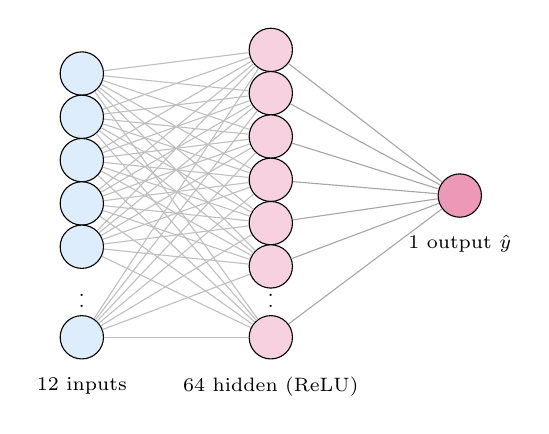
\begin{tikzpicture}[
  neuron/.style={circle, draw, minimum size=0.55cm},
  lbl/.style={font=\scriptsize}
]
\foreach \i in {1,...,5} {\node[neuron, fill=cARC!15] (i\i) at (0, -\i*0.55) {};}
\node[lbl] at (0,-3.4) {$\vdots$};
\node[neuron, fill=cARC!15] (i6) at (0,-3.9) {};
\node[lbl, below=0.1cm of i6] {12 inputs};

\foreach \j in {1,...,6} {\node[neuron, fill=cTIDE!20] (h\j) at (2.4, -\j*0.55+0.3) {};}
\node[lbl] at (2.4,-3.4) {$\vdots$};
\node[neuron, fill=cTIDE!20] (h7) at (2.4,-3.9) {};
\node[lbl, below=0.1cm of h7] {64 hidden (ReLU)};

\node[neuron, fill=cTIDE!45] (o) at (4.8,-2.1) {};
\node[lbl, below=0.1cm of o] {1 output $\hat{y}$};

\foreach \i in {1,...,6} \foreach \j in {1,...,7} \draw[gray!50, thin] (i\i) -- (h\j);
\foreach \j in {1,...,7} \draw[gray!70] (h\j) -- (o);
\end{tikzpicture}
\caption{The network: 12 features $\to$ 64 hidden units with a ReLU (``keep positive values, zero out
negative ones'') $\to$ one predicted reuse-time.}
\end{figure}

\subsection{Turning scores into a decision}
Given the scores $\hat{y}_0,\dots,\hat{y}_n$ for the $n{+}1$ candidates (index 0 is always ARC's own
choice, the oldest key), TIDE does \emph{not} blindly take the maximum. It evicts
\[
\arg\max_i \big(\hat{y}_i - m_i\big), \qquad m_i =
\begin{cases}
0 & i = 0 \text{ (ARC's own candidate)}\\
\delta = 0.1 & i \in \{1,2,3\} \text{ (other tail candidates)}\\
\delta_{\text{far}} = 0.2 & i \text{ is the MRU key or the incoming key}
\end{cases}
\]
The margins $\delta$ and $\delta_{\text{far}}$ mean the model has to be \emph{clearly} more confident
than ARC's own guess before it is allowed to override it, and needs to be even more confident to make the
riskier MRU or bypass choice. These numbers were picked once, by testing a grid of settings across every
trace used in the benchmark, and then fixed for all traces --- nothing here is tuned per trace.

\section{Learning while the cache runs}
This is the part that lets TIDE improve over time instead of being trained once and frozen. The key idea
is: \emph{every candidate the model ever scores eventually gets a correct answer for free}, because the
cache keeps running and either sees that key again or does not.

\begin{figure}[H]
\centering
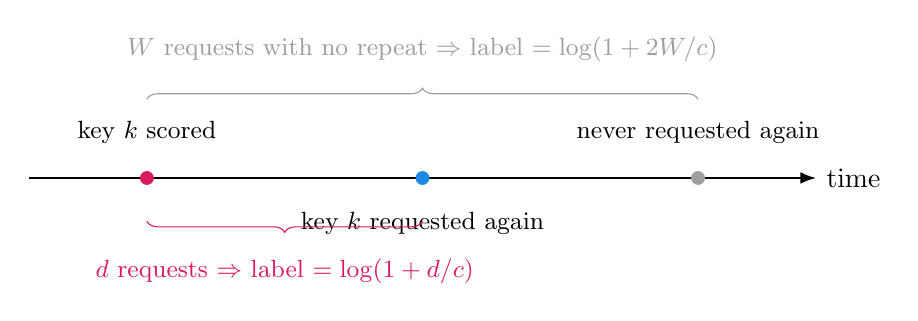
\begin{tikzpicture}[
  ev/.style={circle, fill=cTIDE, minimum size=5pt, inner sep=0pt},
]
\draw[thick, -{Latex[length=2mm]}] (0,0) -- (10,0) node[right] {time};
\node[ev] (t0) at (1.5,0) {};
\node[font=\small, above=0.22cm of t0] {key $k$ scored};
\node[ev, cARC] (t1) at (5,0) {};
\node[font=\small, below=0.22cm of t1] {key $k$ requested again};
\node[ev, cGray] (t2) at (8.5,0) {};
\node[font=\small, above=0.22cm of t2] {never requested again};
\draw[decorate, decoration={brace, amplitude=4pt, mirror}, cTIDE] (1.5,-0.55) -- (5,-0.55)
  node[midway, below=10pt, font=\small] {$d$ requests $\Rightarrow$ label $= \log(1+d/c)$};
\draw[decorate, decoration={brace, amplitude=4pt}, cGray] (1.5,1.0) -- (8.5,1.0)
  node[midway, above=10pt, font=\small] {$W$ requests with no repeat $\Rightarrow$ label $= \log(1+2W/c)$};
\end{tikzpicture}
\caption{Every scored candidate resolves into a training example, one way or the other, with no need for
a human or a special "ground truth" file. The two outcomes (reused after $d$ requests, or censored after
$W$) are alternatives for the same candidate, not two separate events.}
\end{figure}

Concretely (\code{tide.py}, methods \code{\_choose}, \code{access}, \code{\_label}):
\begin{enumerate}
  \item Whenever a candidate is scored (whether or not the model is even switched on yet, see
        \S\ref{sec:coldstart}), its 12 features are copied into a \emph{pending} table, timestamped with
        the current request number $t_0$.
  \item On every later request for key $k$: if $k$ has a pending entry, it is resolved with label
        $\log(1+d/c)$ where $d = t - t_0$ is exactly how many requests it took to come back. This happens
        \emph{even on a cache hit} — resolving labels does not depend on whether the request was a hit or
        a miss.
  \item If $W = 8c$ requests pass with no repeat, the pending entry expires and is resolved as
        \emph{censored}: labelled $\log(1+2W/c)$, the LRB convention of "twice the window", so the model
        learns "very far away" rather than a wrong precise number.
  \item Each resolved (features, label) pair is written into a 32{,}768-row \emph{replay buffer} that
        overwrites its oldest rows once full, so old, possibly outdated patterns are gradually forgotten
        and never pinned forever.
  \item Every 32 new labels, one training step runs: sample 256 random rows from the replay buffer and
        take one Adam optimiser step to reduce the mean-squared error between the network's prediction and
        the true label.
\end{enumerate}

\subsection{The exact training step}
Given a batch of 256 (features, label) pairs $(x_i, y_i)$, the loss is mean squared error,
$\mathcal{L} = \frac{1}{256}\sum_i (\hat{y}_i - y_i)^2$, and every weight is updated with Adam
(Kingma \& Ba, 2015), which keeps a running average of the gradient ($m$) and of its square ($v$) so that
each of the roughly 1{,}600 numbers in the network gets its own, self-adjusting step size:
\[
m \leftarrow 0.9\,m + 0.1\,g \qquad v \leftarrow 0.999\,v + 0.001\,g^2 \qquad
\theta \leftarrow \theta - \frac{\eta}{\sqrt{\hat v} + \varepsilon}\,\hat m
\]
with $\hat m, \hat v$ the usual bias-corrected versions and learning rate $\eta = 10^{-3}$. All four weight
tensors ($W_1$, $b_1$, $w_2$, $b_2$, about 1{,}601 numbers for the default 64 hidden units) are stored in
one flat array so the whole update above is a handful of NumPy vector operations rather than a loop.

\subsection{Cold start: no guessing before there is evidence}\label{sec:coldstart}
TIDE does not turn its model on immediately. It keeps collecting labels and training in the background,
but every eviction is decided exactly as plain ARC would decide it, until \emph{all} of these are true:
\begin{itemize}
  \item at least $W = 8c$ requests have happened (so the "never came back" signal is meaningful), and
  \item at least 2{,}048 labels have been collected (so the replay buffer isn't mostly empty), and
  \item the model is not currently in a fallback cool-down (next section).
\end{itemize}
This means the very first stretch of any trace is identical to plain ARC, and TIDE only starts
overriding decisions once it has real evidence to act on.

\section{The safety net: never much worse than ARC}
A model can be wrong, especially right after the workload changes. TIDE protects against this with a
second, independent copy of plain ARC running silently alongside it (the \emph{shadow}), fed the exact
same requests but never influenced by TIDE's decisions.

\begin{figure}[H]
\centering
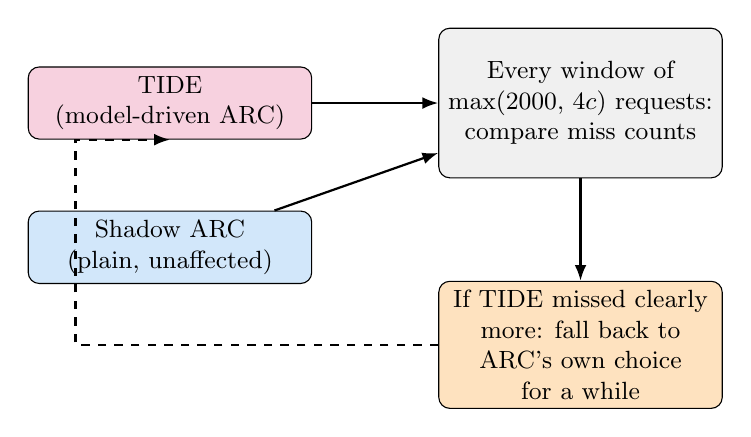
\begin{tikzpicture}[
  box/.style={draw, rounded corners, minimum height=0.9cm, align=center, font=\small},
  arr/.style={-{Latex[length=2mm]}, thick}
]
\node[box, fill=cTIDE!20, minimum width=3.6cm] (tide) {TIDE\\(model-driven ARC)};
\node[box, fill=cARC!20, below=0.9cm of tide, minimum width=3.6cm] (shadow) {Shadow ARC\\(plain, unaffected)};
\node[box, fill=cGray!15, right=1.6cm of tide, minimum width=3.6cm, minimum height=1.9cm] (cmp)
  {Every window of\\$\max(2000,\,4c)$ requests:\\compare miss counts};
\node[box, fill=cOrange!25, below=1.3cm of cmp, minimum width=3.6cm]
  (fb) {If TIDE missed clearly\\more: fall back to\\ARC's own choice\\for a while};
\draw[arr] (tide) -- (cmp);
\draw[arr] (shadow) -- (cmp);
\draw[arr] (cmp) -- (fb);
\draw[arr, dashed] (fb.west) -| ($(tide.south)+(-1.2,0)$) -- (tide.south);
\end{tikzpicture}
\caption{The shadow comparison and fallback loop. The fallback path is dashed because it feeds back into
future decisions, not the current one.}
\end{figure}

Every $\max(2000, 4c)$ requests, TIDE compares its own miss count to the shadow's. If TIDE missed more by
more than $\max(10,\, 1\%$ of the window$)$, it falls back to letting ARC's own rule choose the victim
for a "cool-down" period. If this keeps happening again and again, the cool-down doubles each time
(2, 4, 8, 16 windows, capped), so a workload that keeps confusing the model gets progressively more of
ARC's steady behaviour instead of the model's guesses. If TIDE goes a window without missing more than the
shadow, the failure count relaxes back down, so a temporary rough patch does not permanently poison the
policy. Two details worth being explicit about, since they are easy to get backwards:
\begin{itemize}
  \item The shadow is \emph{only} used to detect regime changes and decide on fallback. It is never used
        as a source of "regime" features for the model itself, because if it were, the model's own past
        mistakes (which count against the real cache, not the shadow) would leak into its inputs.
  \item Label collection and training \emph{continue during fallback}. The model keeps learning even while
        it isn't making decisions, so once the workload settles back down it can immediately re-activate
        with a model that has kept up to date.
\end{itemize}

\section{Putting it together: what happens on one request}
\begin{enumerate}
  \item Advance the clock. Expire any pending candidate snapshot older than $W$ requests (censored
        label). If the requested key has a pending snapshot, resolve it with the true gap $d$.
  \item Update that key's history record (last three gaps, smoothed average, three decayed counters,
        total count).
  \item Feed the request to the shadow ARC (for later comparison only).
  \item Run ARC's normal logic: hit in T1 or T2, or a ghost hit in B1/B2 (which updates $p$), or a genuine
        miss.
  \item If a miss requires an eviction: ARC's rule (unchanged) decides the list; TIDE scores up to 6
        candidates from that list (Section 3) and, if the model is switched on, evicts the one with the
        lowest trusted score; otherwise it falls back to ARC's own oldest-item choice.
  \item Every 32 newly resolved labels, run one training step (Section 5.1).
  \item Every $\max(2000,4c)$ requests, compare against the shadow and update the fallback state
        (Section 6).
\end{enumerate}

\section{A worked mini-example}
Suppose the cache holds keys $\{5, 9, 12, 20\}$ in T1's cold-to-hot order, cache size $c=4$, and key 20 is
the most-recently-used key of T1. A miss now forces an eviction from T1. The four tail candidates are
$5, 9, 12, 20$ (note: 20 also happens to be the MRU key here since T1 has only 4 items, so no separate
MRU candidate is added). Suppose their fast decayed counters and last-gap history give the model these
predicted values (already net of the margin, for illustration):
\[
\hat{y}_5 = 0.9 \quad(\text{not requested in ages, low frequency})
\qquad
\hat{y}_9 = 2.4 \quad(\text{part of a big loop, due back in a long time})
\]
\[
\hat{y}_{12} = 0.3 \quad(\text{steadily popular, likely requested very soon})
\qquad
\hat{y}_{20} = 1.1 \quad(\text{ARC's own pick, the plain LRU choice})
\]
With margins $\delta = 0.1$ applied to candidates 9, 12, 20 (all "other tail" candidates) and none to the
ARC default (index 0, key 5 in this ordering): $5.90,\ 9\!:2.30,\ 12\!:0.20,\ 20\!:1.00$. The
highest adjusted score is key 9's, so TIDE evicts key 9, not key 5 (ARC's own pick) and not the
still-frequently-needed key 12. Some time later, whichever of these keys is next requested resolves that
key's label with the true gap, and the network is nudged toward whichever prediction turns out to have
been right.

\section{Why not PyTorch or TensorFlow}
The network here has about 1{,}600 numbers and is called on 4--6 rows at a time, thousands of times per
second, inside a single-threaded cache simulator. A deep-learning framework's per-call overhead (tens of
microseconds just to enter and leave the framework) would dominate the actual arithmetic, which NumPy
does directly with essentially no overhead. Bringing in a roughly gigabyte dependency to save about 20
lines of hand-written gradient and Adam code (which is fully tested, see
\code{test\_tide.py::test\_grad}, a numerical gradient check) is not worth it here. It would be
worth it if the network grew much larger, or for an \emph{offline} teacher model such as a small
transformer trained once on a GPU and then distilled into a model this size for the actual cache --- an
idea discussed as "Option C" in the project's design document, \code{REPLAN.md}.

\section{Headline results}
Full detail, every trace and cache size, is in the companion document \code{report.pdf}. In short, on a
43-cell benchmark (12 real/synthetic traces $\times$ 3 cache sizes, plus 3 generated 1-million-request
trend traces $\times$ 3 cache sizes), averaged over \Seeds{} random seeds:
\begin{itemize}
  \item TIDE has the best mean normalized hit rate of the compared policies: \NormTIDE{} vs.\ \NormARC{}
        for ARC and \NormSthree{} for S3-FIFO (0 = no better than the simplest policy, LRU; 1 = as good as
        the theoretical optimum, Belady's algorithm, which requires knowing the future).
  \item TIDE has the single highest hit rate in \WinsTIDE{} of \NCells{} cells, and is at least as good as
        plain ARC in \GeARC{} of them.
  \item On the loop-shaped ``adversarial'' trace, TIDE turns a \textbf{0\%} hit rate into roughly
        \textbf{\AdvGain} percentage points, purely through the bypass mechanism in Section 3.
  \item A decision takes about 15\,\textmu s at the median and never took more than \PNineNineMax\,\textmu
        s at the 99th percentile in these benchmarks; a cache \emph{hit} never touches the model at all.
\end{itemize}

\end{document}
